\newpage


\section{Hyper-parameters}\label{sec:hyper-parameters}

Proposed genetic algorithm~\ref{alg:genetic} has eight hyperparameters.
They are described in table~\ref{tab:hyperparameters-description}.
The rest of the sections discuss these hyperparameters further and tries to find their reasonable values.

Hyperparameter testing is performed by changing only the hyperparameter under test.
Hyperparameters not under test are identical to the values in listing~\ref{lst:computation-submission-dataset}.
The exceptions are penalization constants $\lambda, \gamma$ (eq.~\ref{eq:objective}), and \verb|populationSize|.
Penalization constants are set to the length of the layout diagonal (see~\ref{subsec:overlapping-penalization-constant}).
Population size is set to $50N$, where $N$ is the size of the instance.
The reason for choosing such parameters as base parameters for testing
is preliminary results (not presented in this thesis), which proved correct in many cases.

To achieve the statistical significance of the results presented in this section, each computation (sec.~\ref{sec:implementation}) is submitted five times with a different random seed.
Presented values are thus an average from five samples.

\begin{table}[h!]
    \caption[Hyperparameters of the genetic algorithm]{Hyperparameters of the genetic algorithm~\ref{alg:genetic}}
    \label{tab:hyperparameters-description}
    \begin{tabular}{ll}
        \hline
        \textbf{Hyperparameter}   & \textbf{Description}                                       \\ \hline
        \verb|maxNumberOfIter|    & maximum number of iterations                               \\ \hline
        \verb|populationSize|     & population size                                            \\ \hline
        \verb|maximumWildCardCount| & \begin{tabular}[c]{@{}l@{}}
                                          limit on the maximum number of $*$ cut types\\ produced by $OR_{prob}$ decoding
        \end{tabular} \\ \hline
        \verb|orientationWeights| & penalization vector $P$ from eq.~\ref{eq:crossover-orprob} \\ \hline
        \verb|populationDivisionCounts| & \begin{tabular}[c]{@{}l@{}}
                                              reproductive plan ratios\\ (left part of fig.~\ref{fig:population-schema})
        \end{tabular} \\ \hline
        \verb|initialPopulationDivisionCounts| &
        \begin{tabular}[c]{@{}l@{}}
            initial population ratios\\ (right part of fig.~\ref{fig:population-schema})
        \end{tabular} \\ \hline
        \verb|overlappingPenalizationConstant| &
        \begin{tabular}[c]{@{}l@{}}
            overlapping paintings penalization\\ parameter $\lambda$ from eq.~\ref{eq:objective}
        \end{tabular} \\ \hline
        \verb|outsideOfAllocatedAreaPenalizationConstant| &
        \begin{tabular}[c]{@{}l@{}}
            outside of allocated area penalization\\ parameter $\gamma$ from eq.~\ref{eq:objective}
        \end{tabular} \\ \hline
    \end{tabular}
\end{table}

\subsection{Max number of iter}\label{subsec:max-number-of-iter}
Hyperparameter \verb|maxNumberOfIter| determines the number of iterations in the genetic algorithm~\ref{alg:genetic}.

Results for two random instances are in figure~\ref{fig:hyperparameters-max-number-of-iter}.
We can see the initial decrease of the average population objective for both random instances.
Between iterations 100 and 150, decreasing trend and fluctuations stop.

The conclusion is that at least 150 iterations are needed before the average population objective
stops decreasing rapidly.

\subsection{Population size}\label{subsec:population-size}

Hyperparameter \verb|populationSize| is calculated as $kN$, where $k$ is \definice{population scaling factor}
and $N$ is instance size.
It determines the population size that is linear to the instance size.

Results for two random instances are in figure~\ref{fig:hyperparameters-population-size}.
We can see that scaling factor $10$ does not allow
the population objective average to decrease to the levels comparable to scaling factors $50$ and $100$.
It might imply that the scaling factor $10$ cannot represent knowledge gathered over time
in the genetic algorithm or that more iterations are needed.

The conclusion is that using scaling factor between $50$ and $100$ is sufficient, with bias towards $100$
for obtaining better average objective performance.
However, increasing the scaling factor leads to slower computation speed as every population contains
more individuals for which genetic operators and reproductive plan must be computed.

\subsection{Maximum wild card count}\label{subsec:maximum-wild-card-count}
Hyperparameter \verb|maximumWildCardCount| limits the maximum number of $*$ cut types produced by $OR_{prob}$ decoding (subsec.~\ref{subsec:individual-decoding}).
Keeping this hyperparameter low or even setting it to zero is recommended.
The reason is that if it is high, computation time increases as $*$ spreads in the population.
For example, consider an individual whose orientation vector is solely composed of $*$ cut types.
If the size of that vector is $n$, individual decodes to $2^n$ resolved slicing trees as seen in figure~\ref{fig:layout-construction-steps}.

Results for random\_10 instance are in figure~\ref{fig:hyperparameters-maximum-wild-card-count}.
On the top sub-figure, we can see that the average population objective does not decrease rapidly for any limit on the wildcard cut type.
However, there is a slight advantage for the maximum wild card count equal to one.
It might be caused by using wildcard penalization $0.5$ (listing~\ref{lst:computation-submission-dataset})
that does not allow the spread of the wildcard in the population.

On the bottom sub-figure, we can see the computation speed as the limit on the wildcard cut type increases.
It grows linearly up to the maximum wild card count of eight, and then the increase stops.
It might be because the wildcard penalization $0.5$ does not
allow the wildcard cut type to spread over the maximum wildcard count of eight.
Another reason might be computational anomalies caused by high-memory consumption as the maximum wild card count increases.

The conclusion is that (a) the maximum wild card count for wildcard penalization $0.5$
performs similarly for all values, with a slight performance gain if using a maximum wild card count equal to one,
and (b) computation time is linear with increasing maximum wild card count and wildcard penalization $0.5$.

\subsection{Orientation weights}\label{subsec:orientation-weights}
Hyperparameter \verb|orientationWeights| determines the bias towards the type of cut ($H$, $V$, $*$, see~\ref{subsec:individual-decoding}) \textit{during crossover}.
The orientation penalization vector $P$ from eq.~\ref{eq:crossover-orprob} contains the penalization value for each cut type.
In this thesis, only penalization for the wildcard cut type $*$ is tested, as there is no need to penalize or have a preference for $H$ or $V$ cut types.
Recall that the hyperparameter \verb|maximumWildCardCount| is \textit{set to one}, as described at the beginning of the section and showed in listing~\ref{lst:computation-submission-dataset}.

Performance results for two random instances are in figure~\ref{fig:hyperparameters-orientation-weights}.
We can see that for random\_10 instance,
weight does not significantly influence the average population objective, and after iteration 250, differences become negligible.
However, for random\_20 instance,
weight one (no penalization) has a faster-decreasing trend and produces a population with a better average population objective.

The reason for better average performance at larger instance with weight one (no penalization) might
be that search space increases exponentially (there are at least $2^{N-1}$ different unresolved slicing trees for instance of size $N$) and the introduction of wildcard cut type $*$ starts to manifest itself
at larger instances.

Results for the number of wildcard cut types $*$ at the best individual at each iteration are in
figure~\ref{fig:hyperparameters-orientation-weights-wildcard-cut-type-spread}.
We can see that for the random\_10 instance, weights below one have less than one wildcard on average.
However, on average, there are between three and four wildcards for a weight equal to one (no penalization).
Similar can be seen for random\_20 instance.

The reason why there are wildcards present in the figure~~\ref{fig:hyperparameters-orientation-weights-wildcard-cut-type-spread}
even for weight equal to zero (maximal penalization) is that wildcard can be introduced to a chromosome by mutation
or injection random individuals (see reproductive plan~\ref{subsec:reproductive-plan}).
Penalization described only applies to the crossover.

First conclusion it that (a) smaller instances, such as random\_10, do not benefit from the introduction of wildcard cut type $*$,
and (b) bigger instances, such as random\_20, benefit from no penalization by having a faster-decreasing trend and producing a better average population.

Second conclusion is that if we want to be certain that wildcard cut type $*$ is contained in the best individual at each iteration,
wild card orientation weight must be set close to one.

\subsection{Population division counts}\label{subsec:population-division-counts}
Hyperparameter \verb|populationDivisionCounts| configures ratios in the reproductive plan (subsec.~\ref{subsec:reproductive-plan}).
It influences how the next generation is created in the genetic algorithm~\ref{alg:genetic}
by setting (a) how many elite individuals are copied, (b) how many children are created using a crossover operator,
(c) how many mutants are created using a mutation operator, (d) how many tournament winners are included,
and (e) how many random individuals are injected.

Performance results for two random instances are in figure~\ref{fig:hyperparameters-population-division-counts}.
We can see that results do not differ for the smaller or larger instance.
The best reproductive plan strategy is achieved without changing population division hyperparameters from listing~\ref{lst:computation-submission-dataset}.
That means elitism and randomly injected individuals are present.
Additionally, we can see that the cause of good performance is the elitism strategy,
as removing randomly generated individuals does not significantly improve performance.

The reason why the use of elitism is important to obtain good results might be the implementation of the crossover operator (subsec.~\ref{subsec:crossover}).
Crossover adds weights $w_A$ and $w_B$ to each parent based on their objective value.
It means that if $w_A \gg w_B$, the offspring is a sample from the search space close to the parent $A$ or nearly identical to $A$.
On the other hand, if the weights are similar and each parent represents a different (sub)-optimal solution,
the transfer of information does not happen, and the offspring is no better than a randomly generated individual.
Elitism avoids crossover by directly copying the best individuals without any modification.
It leads to keeping track of multiple (sub)-optimal solutions simultaneously.
In addition, each time a crossover is applied, one parent is selected from the elite pool,
which supports intensification.

On the other hand, removing elitism produces the worst results.
The reason might be the inability to keep track of competing (sub)-optimal and the fast spread of the first
\definice{macho individual}, an individual that performs significantly better than everyone else.
Without elitism, the most significant way to keep track of found (sub)-optimal solutions is through crossover.
Crossover chooses parents randomly from the average pool, which does not give any constraint on the weights $w_A$ and $w_B$.
Additionally, as mentioned in the previous paragraph, similar weights for two different parents produce no better offspring than randomly generated individuals.
It means that most offspring do not perform well.
On the other hand, as soon as the macho individual appears as the parent in the crossover, the offspring is effectively a copy of a macho individual.
Then, if the macho individual is randomly chosen more than once as a parent in a crossover, it rapidly spreads and takes over the whole population.
The chance of macho-individual taking over the population with elitism is decreased as it deliberately keeps track of multiple performant individuals,
making it harder for the macho individual to spread.

The conclusion is that  using elitism is essential for obtaining good painting placement solutions
as it can keep track of multiple (sub)-optimal solutions simultaneously.


\subsection{Initial population division counts}\label{subsec:initial-population-division-counts}
Hyperparameter \verb|initialPopulationDivisionCounts| configures generation ratios of the initial population (left part of fig.~\ref{fig:population-schema}).
It consists of randomly generated and greedily generated individuals.

Performance results for two random instances are in figure~\ref{fig:hyperparameters-initial-population-division-counts}.
The different ratios' results do not significantly differ.

The conclusion is that hyperparameter \verb|initialPopulationDivisionCounts| does not significantly affect the obtained results.

\subsection{Overlapping penalization constant}\label{subsec:overlapping-penalization-constant}

Hyperparameter \verb|overlappingPenalizationConstant| is the penalization constant $\lambda$ from eq.~\ref{eq:objective}.
It penalizes individuals that represent solutions with paintings that overlap.
It is calculated as $kD$, where $k$ is a diagonal multiple and $D$ is the length of a diagonal in a layout.
Diagonal length $D$ for a layout with width $W$ and height  $H$ is $\sqrt{W^2 + H^2}$.

Results of the average overlapping count for the best individual at each iteration are in figure~\ref{fig:hyperparameters-overlapping-penalization-constant}.
We can see that the diagonal multiple $k$ with values $0.5$ and $1.0$ is not high enough to remove overlapping paintings from the population.
However, values $0.2$ and higher perform similarly in reducing the overlapping paintings.

The conclusion is that hyperparameter \verb|overlappingPenalizationConstant| should be set at least to
two times the diagonal length of the layout to sufficiently penalize individuals that represent solutions with overlapping paintings.

\subsection{Outside of allocated area penalization constant}\label{subsec:outside-of-allocated-area-penalization-constant}
Hyperparameter \verb|outsideOfAllocatedAreaPenalizationConstant| is the penalization constant $\gamma$ from eq.~\ref{eq:objective}.
It penalizes paintings that are placed outside their allocated area (see fig.~\ref{fig:allocated-area} and subsec.~\ref{subsec:placement-heuristic}).
It is calculated identically as \verb|overlappingPenalizationConstant|.
That is, as $kD$, where $k$ is a diagonal multiple and $D$ is the length of a diagonal in a layout.

Results of the average number of paintings outside their allocated area
for the best individual at each iteration are in table~\ref{tab:hyperparameters-outside-of-allocated-area-penalization-constant}.
We can see that diagonal multiple cannot force the creation of the allocated space that would fit most paintings.
In addition, there are a few percentage points drops in favor of the larger instance.
The reason might be that it has more degrees of freedom, i.e., a number of cuts,
and can create more fitting slicing layouts.

However, the failure of \verb|outsideOfAllocatedAreaPenalizationConstant| hyperparameter to force
the creation of sufficient allocated space in most cases is not that important.
The reason is the placing heuristic (subsec.~\ref{subsec:placement-heuristic})
tries to place the painting at several placement points in the allocated area (see fig.~\ref{fig:allocated-area}).
It can thus balance the few paintings that have been allocated sufficient area to avoid overlapping with other paintings
and account for other parts of the objective function.

The conclusion is that hyperparameter \verb|outsideOfAllocatedAreaPenalizationConstant| is the least
important and might be left out by setting it to zero to save computation time.

\begin{table}[h!]
    \caption{Percentage of paintings placed outside allocated area}
    \label{tab:hyperparameters-outside-of-allocated-area-penalization-constant}
    \shorthandoff{-}
    \begin{threeparttable}
        \begin{tabular}{lll}
            \cline{1-3}
            & \multicolumn{2}{c}{\textbf{Instance}} \\ \cline{2-3}
            \textbf{\begin{tabular}[c]{@{}l@{}}
                        Diagonal\\ multiple
            \end{tabular}} & \multicolumn{1}{c}{random\_10} & \multicolumn{1}{c}{random\_20} \\ \hline
            0              & 99.6                           & 93.3                           \\ \hline
            0.5            & 99.6                           & 94.1                           \\ \hline
            1              & 98                             & 92.5                           \\ \hline
            2              & 97.4                           & 95.9                           \\ \hline
            3              & 98.9                           & 91.7                           \\ \hline
            4              & 99.8                           & 94.9                           \\ \hline
            10             & 99.7                           & 96.1                           \\ \hline
            50             & 98.6                           & 97.8                           \\ \hline
        \end{tabular}
        \begin{tablenotes}
            \small
            \item Percentage is averaged over all iterations for the best individual at each iteration.
        \end{tablenotes}
    \end{threeparttable}
    \shorthandon{-}
\end{table}

\begin{figure}[h!]
    \centering
    \subfloat{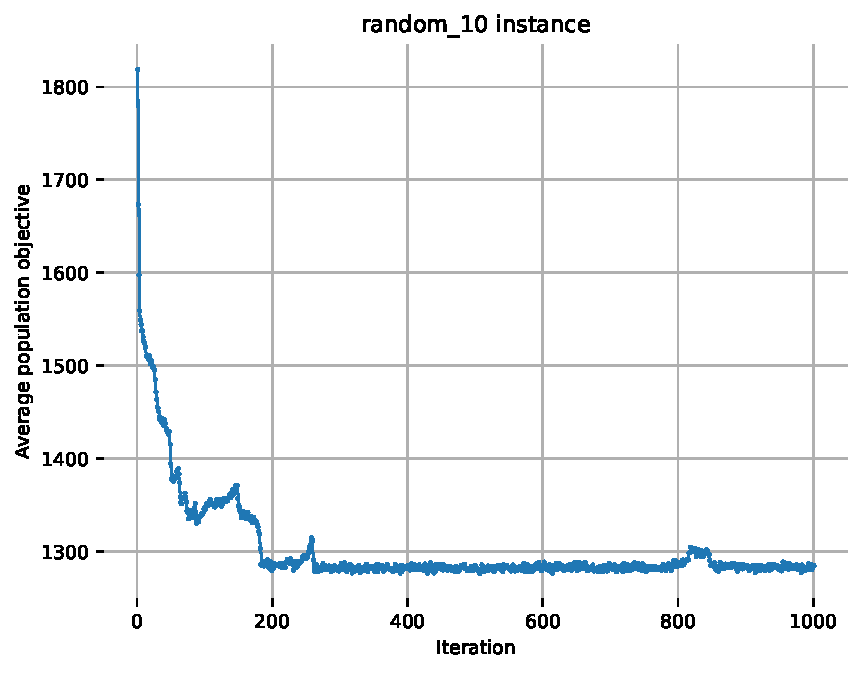
\includegraphics[width=0.8\textwidth]{hyperparameters/max_number_of_iter_random_10}\label{subfig:hyperparameters-max-number-of-iter-random-10}}

    \subfloat{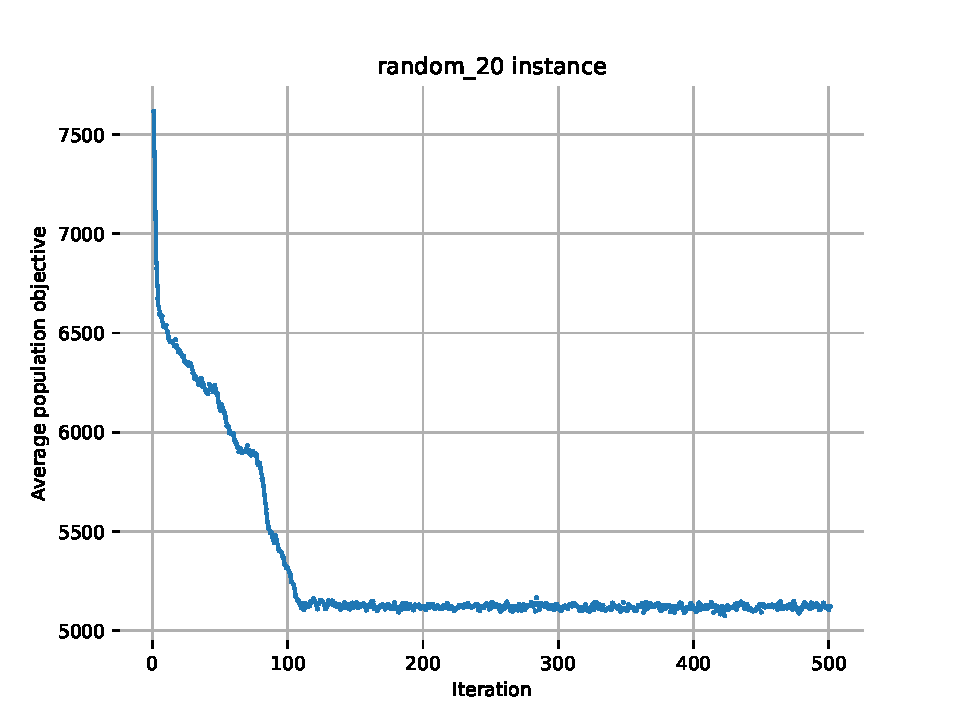
\includegraphics[width=0.8\textwidth]{hyperparameters/max_number_of_iter_random_20}\label{subfig:hyperparameters-max-number-of-iter-random-20}}
    \caption[Testing maximum number of iterations]
    {Testing maximum number of iterations at two random instances.}
    \label{fig:hyperparameters-max-number-of-iter}%
\end{figure}

\begin{figure}[h!]
    \centering
    \subfloat{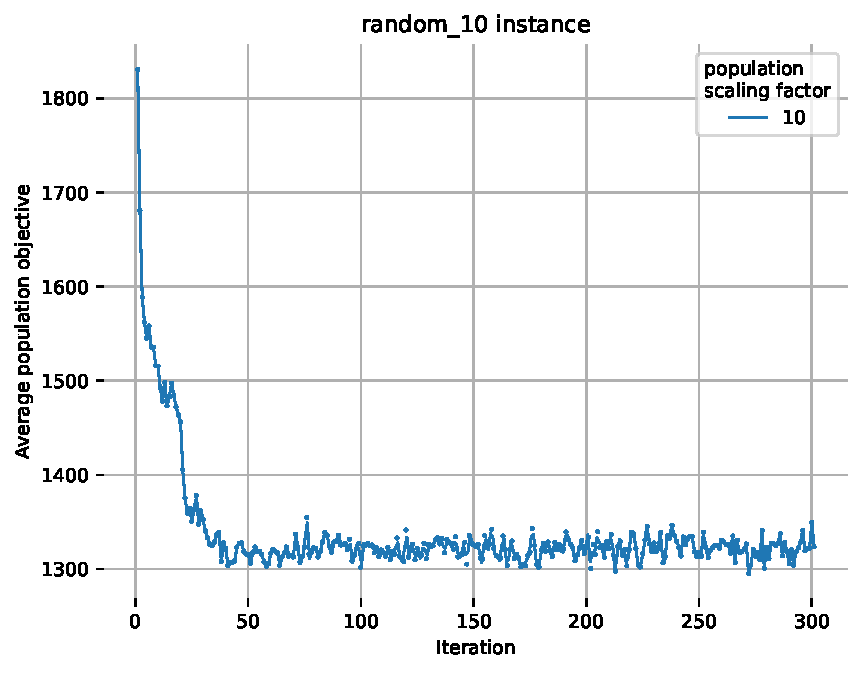
\includegraphics[width=0.8\textwidth]{hyperparameters/population_size_random_10}\label{subfig:hyperparameters-population-size-random-10}}

    \subfloat{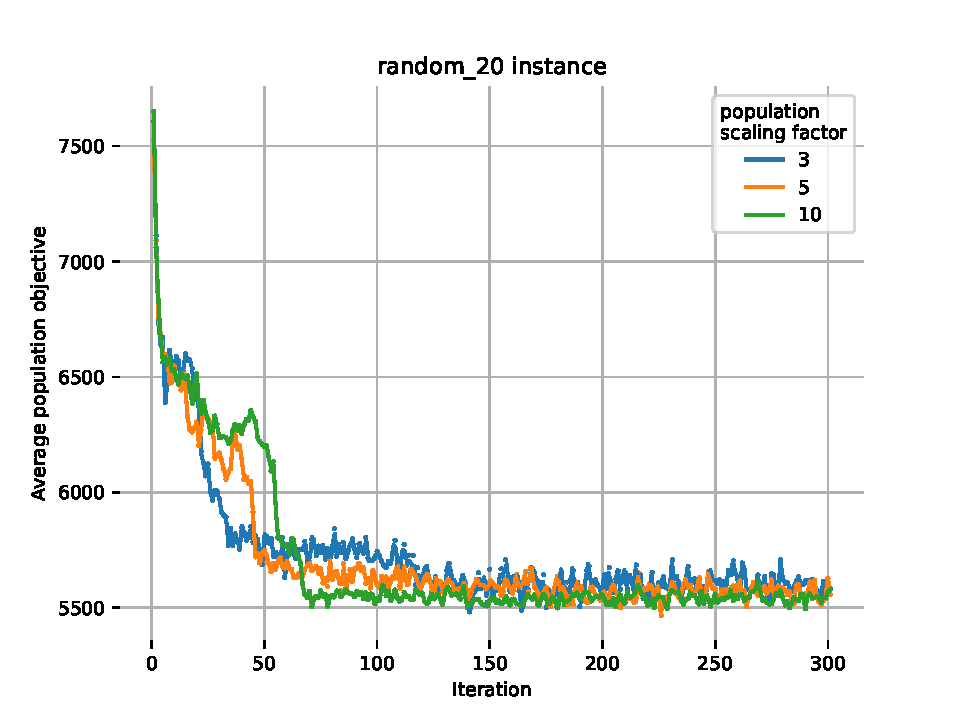
\includegraphics[width=0.8\textwidth]{hyperparameters/population_size_random_20}\label{subfig:hyperparameters-population-size-random-20}}
    \caption[Testing population scaling factor]
    {Testing population scaling factor at two random instances.
    The population size is $kN$ for population scaling factor $k$ and instance of size $N$. }
    \label{fig:hyperparameters-population-size}%
\end{figure}

\begin{figure}[h!]
    \centering
    \subfloat{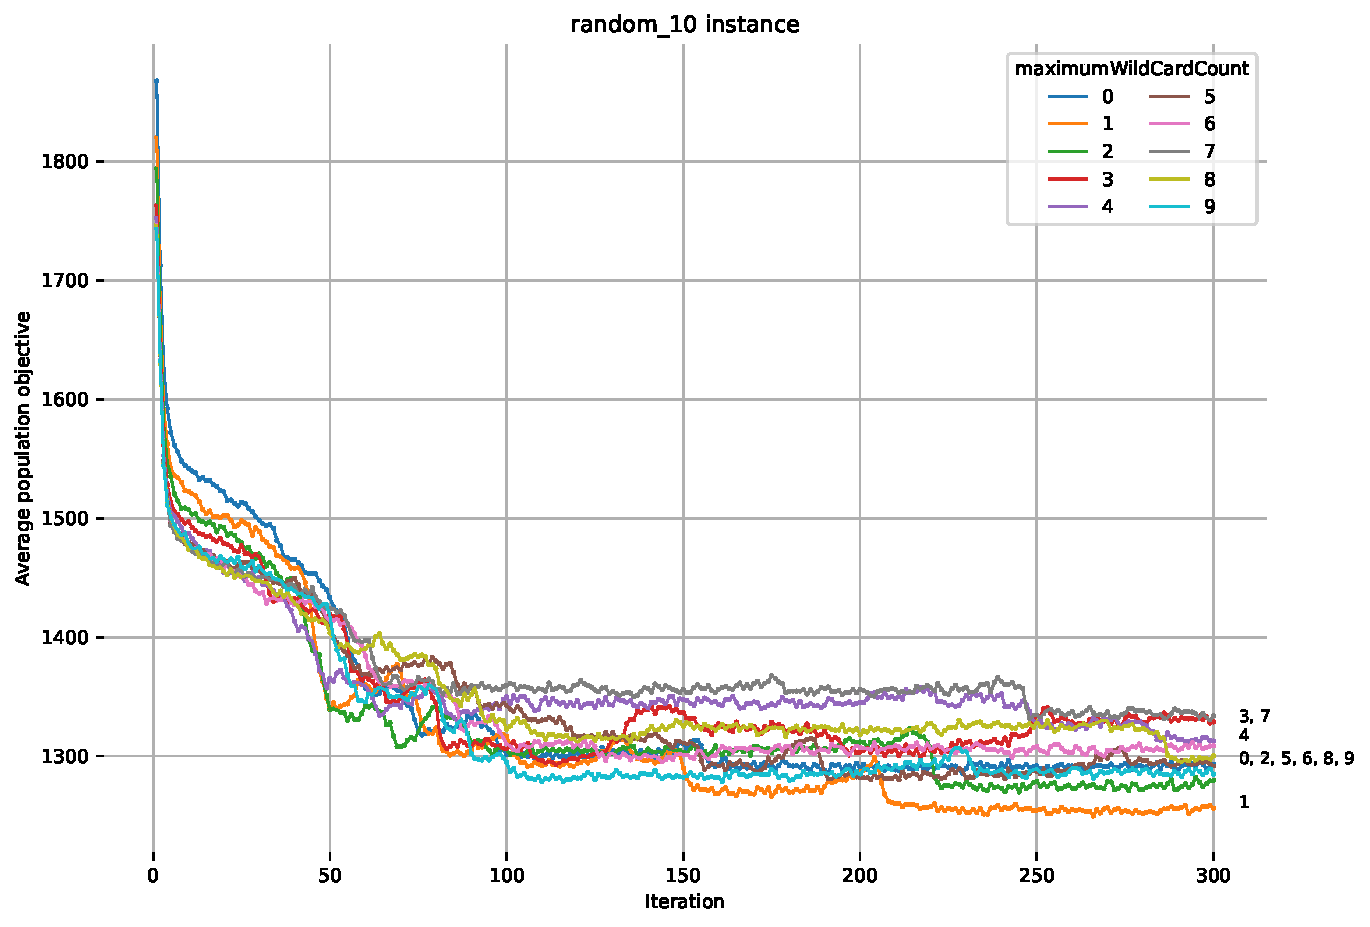
\includegraphics[width=0.8\textwidth]{hyperparameters/maximum_wild_card_count_performance_random_10}\label{subfig:hyperparameters-maximum-wild-card-count-performance}}

    \subfloat{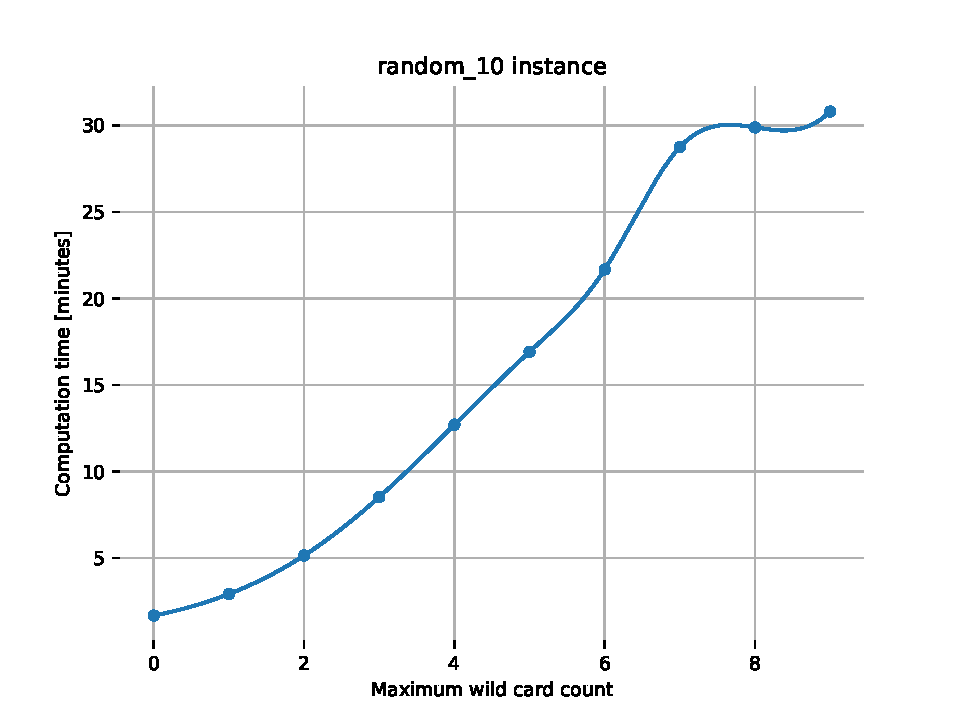
\includegraphics[width=0.8\textwidth]{hyperparameters/maximum_wild_card_count_computation_time_random_10}\label{subfig:hyperparameters-maximum-wild-card-count-computation-speed}}
    \caption[Testing maximum wild card count]
    {Testing increasing maximum wild card count. Performance (top) and computation speed (bottom).}
    \label{fig:hyperparameters-maximum-wild-card-count}%
\end{figure}


\begin{figure}[h!]
    \centering
    \subfloat{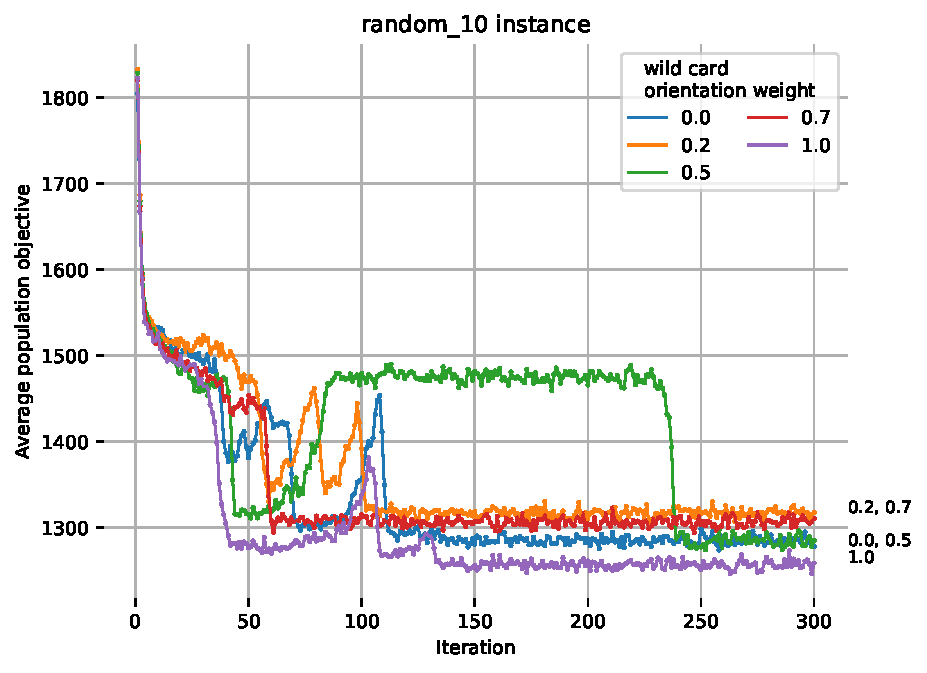
\includegraphics[width=0.8\textwidth]{hyperparameters/orientation_weights_random_10}\label{subfig:hyperparameters-orientation-weights-random-10}}

    \subfloat{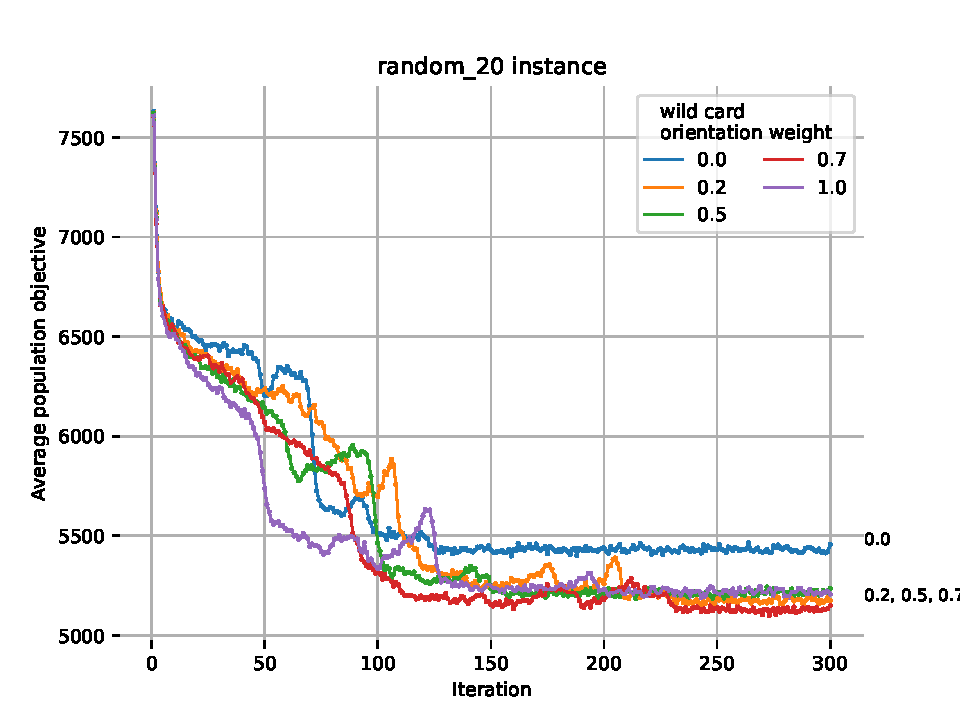
\includegraphics[width=0.8\textwidth]{hyperparameters/orientation_weights_random_20}\label{subfig:hyperparameters-orientation-weights-random-20}}
    \cprotect\caption[Testing orientation weights performance]
    {Testing performance of orientation weight for a wildcard cut type $*$ at two random instances.
    Hyperparameter \verb|maximumWildCardCount| is 1.}
    \label{fig:hyperparameters-orientation-weights}%
\end{figure}

\begin{figure}[h!]
    \centering
    \subfloat{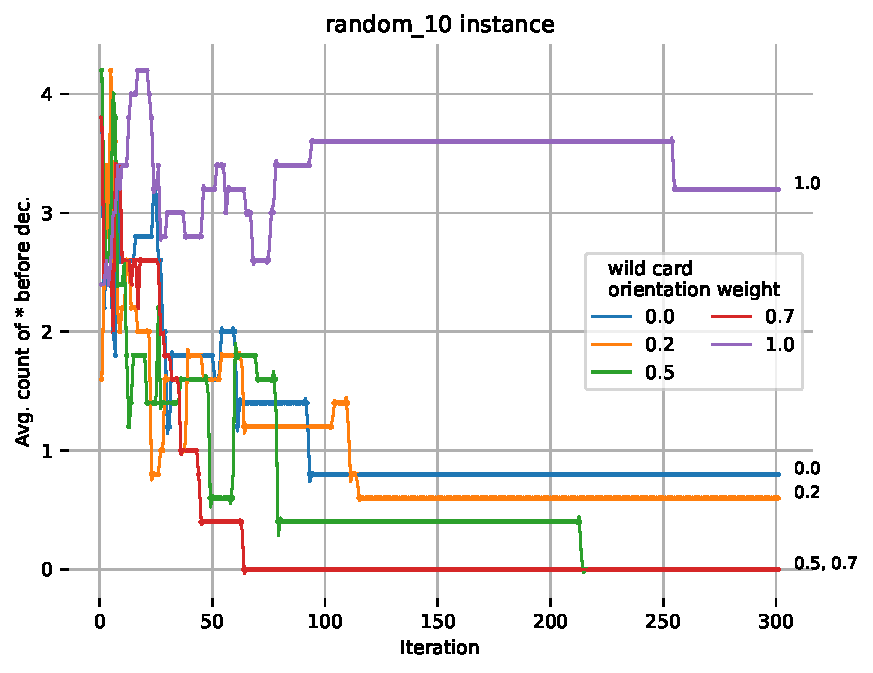
\includegraphics[width=0.8\textwidth]{hyperparameters/orientation_weights_wildcard_cut_type_spread_random_10}\label{subfig:hyperparameters-orientation-weights-wildcard-cut-type-spread-random-10}}

    \subfloat{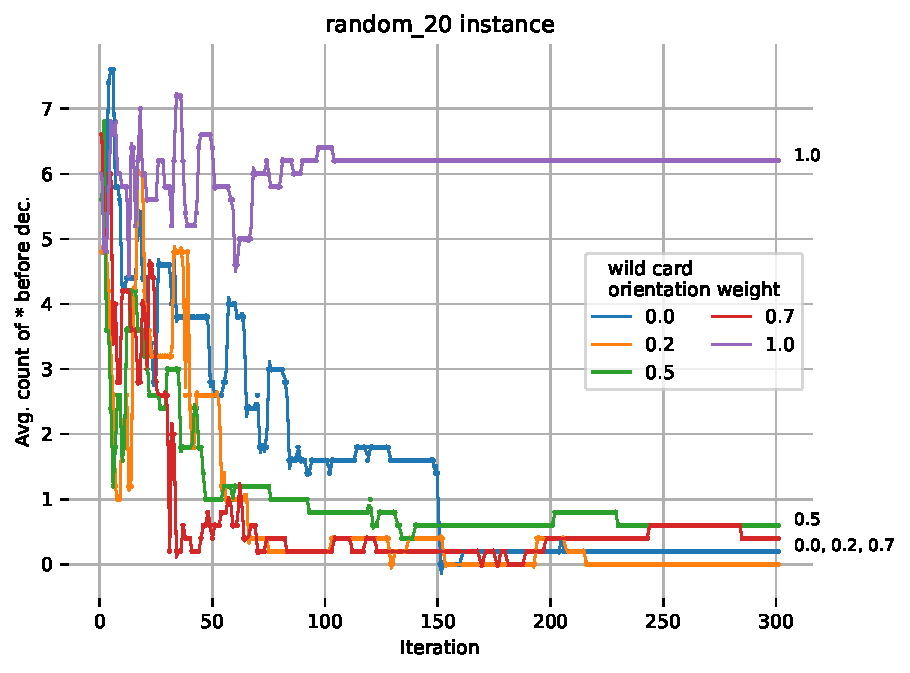
\includegraphics[width=0.8\textwidth]{hyperparameters/orientation_weights_wildcard_cut_type_spread_random_20}\label{subfig:hyperparameters-orientation-weights-wildcard-cut-type-spread-random-20}}
    \cprotect\caption[Testing wildcard spread]
    {Testing wildcard spread at two random instances.
    Each iteration shows average count of wildcard cut type $*$ at best individual for different values of wild card orientation weights.
    Hyperparameter \verb|maximumWildCardCount| is 1.}
    \label{fig:hyperparameters-orientation-weights-wildcard-cut-type-spread}%
\end{figure}

\begin{figure}[h!]
    \centering
    \subfloat{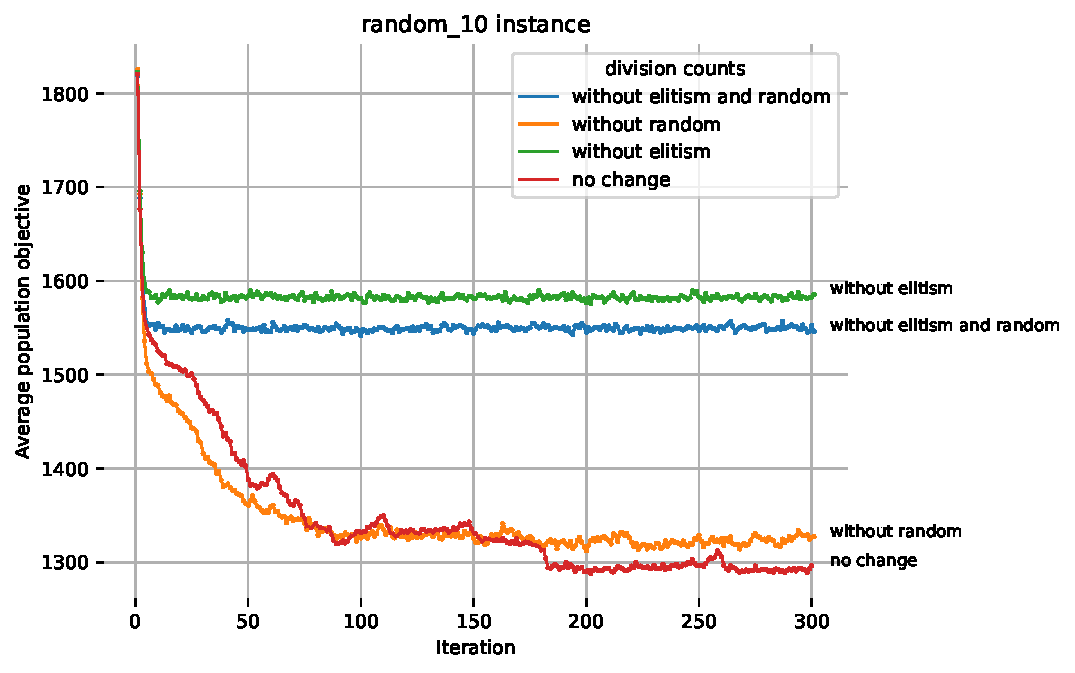
\includegraphics[width=0.8\textwidth]{hyperparameters/population_division_counts_random_10}\label{subfig:hyperparameters-population-division-counts-random-10}}

    \subfloat{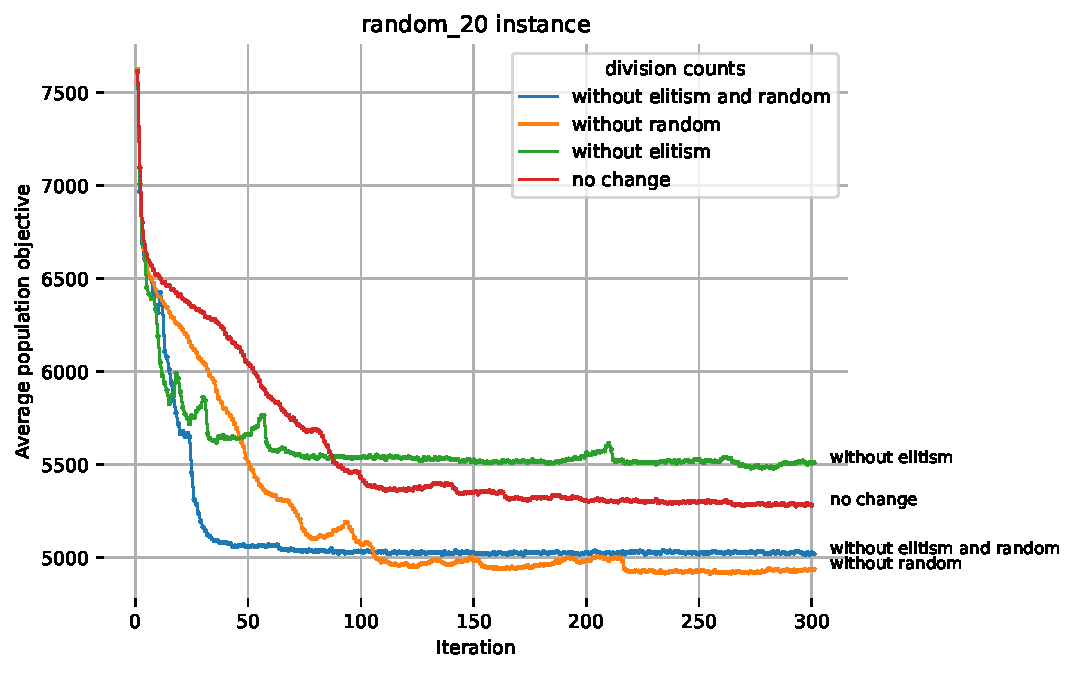
\includegraphics[width=0.8\textwidth]{hyperparameters/population_division_counts_random_20}\label{subfig:hyperparameters-population-division-counts-random-20}}
    \caption[Testing population division counts]
    {Testing population division counts at two random instances. Four variants are displayed.
    The first does not use elitism.
    The second does not inject random individuals.
    The third combines the first and second, and the last does not change the population division counts as described in listing~\ref{lst:computation-submission-dataset}.}
    \label{fig:hyperparameters-population-division-counts}%
\end{figure}

\begin{figure}[h!]
    \centering
    \subfloat{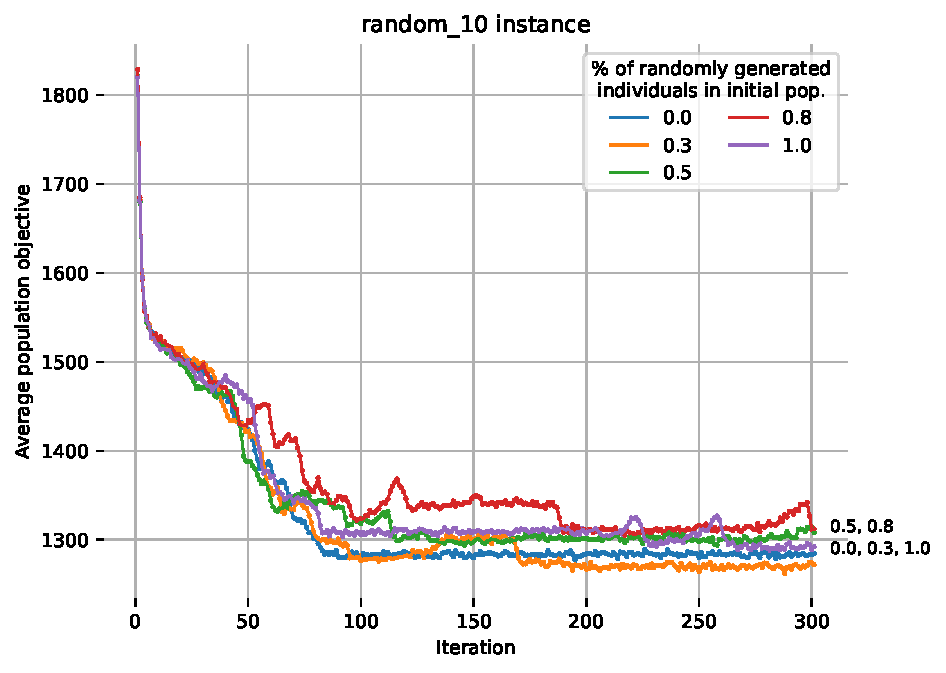
\includegraphics[width=0.8\textwidth]{hyperparameters/initial_population_division_counts_random_10}\label{subfig:hyperparameters-initial-population-division-counts-random-10}}

    \subfloat{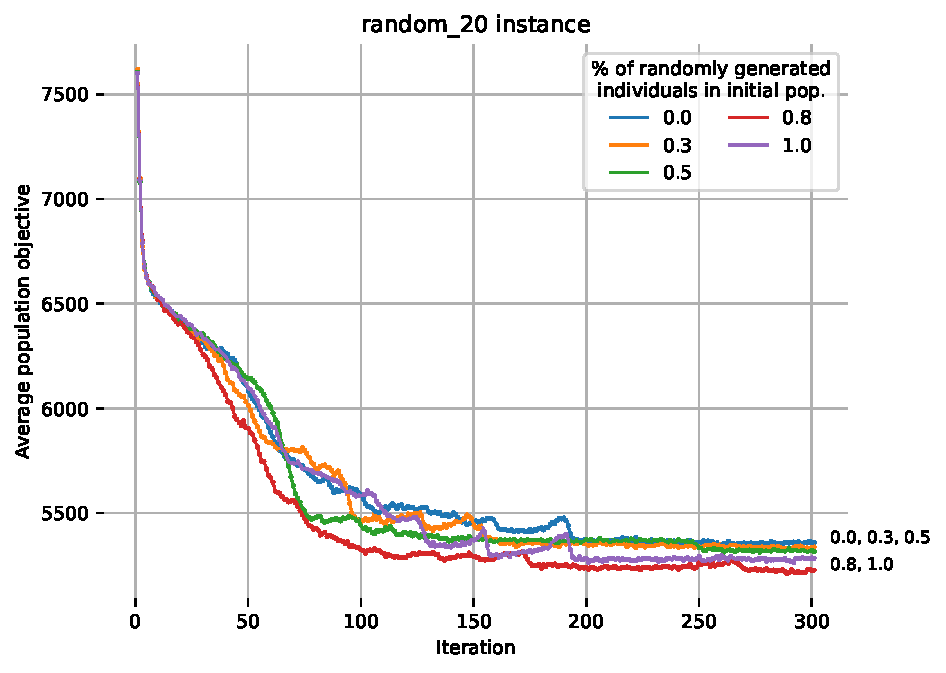
\includegraphics[width=0.8\textwidth]{hyperparameters/initial_population_division_counts_random_20}\label{subfig:hyperparameters-initial-population-division-counts-random-20}}
    \caption[Testing initial population division counts]
    {Testing initial population division counts at two random instances.
    Initial population consists of randomly generated and greedily generated individuals (left part of fig.~\ref{fig:population-schema}).}
    \label{fig:hyperparameters-initial-population-division-counts}%
\end{figure}

\begin{figure}[h!]
    \centering
    \subfloat{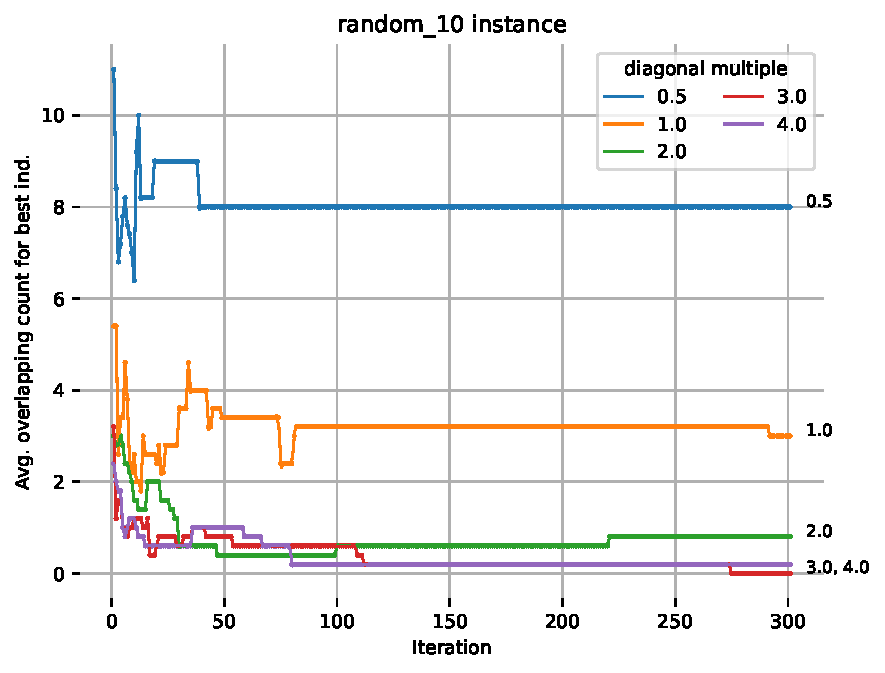
\includegraphics[width=0.8\textwidth]{hyperparameters/overlapping_penalization_constant_random_10}\label{subfig:hyperparameters-overlapping-penalization-constant-random-10}}

    \subfloat{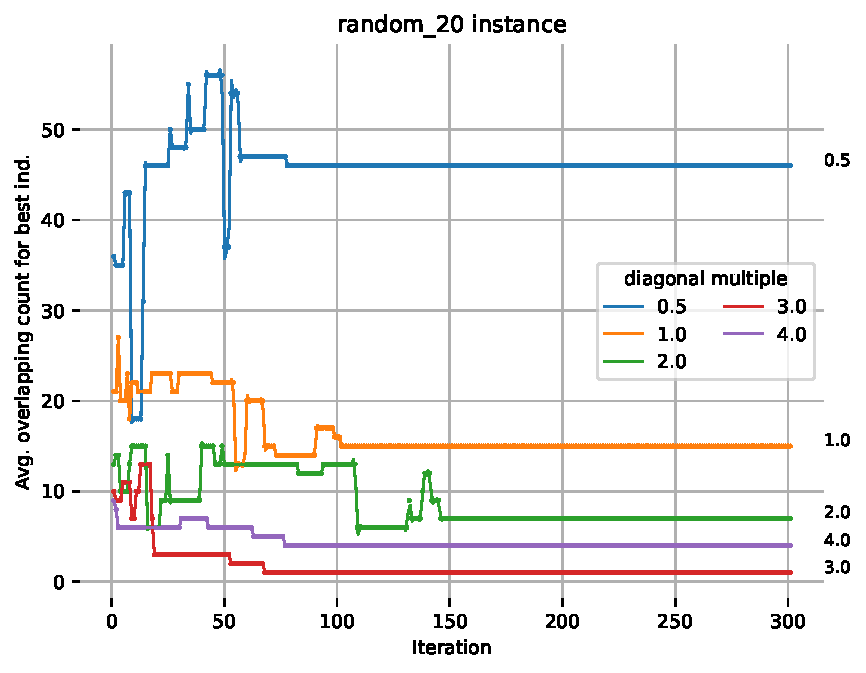
\includegraphics[width=0.8\textwidth]{hyperparameters/overlapping_penalization_constant_random_20}\label{subfig:hyperparameters-overlapping-penalization-constant-random-20}}
    \caption[Testing overlapping penalization constant]
    {Testing overlapping penalization constant $\lambda$ (eq.~\ref{eq:objective}) at two random instances.
    It is determined as $kD$, where $k$ is a diagonal multiple and $D$ is the length of a diagonal in a layout.
    Graphs show the average overlapping count for the best individual at each iteration.}
    \label{fig:hyperparameters-overlapping-penalization-constant}%
\end{figure}


